TODO potevamo dire alla select di prendere il lock ma questo modificava troppo la logica del kernel, tenere un approccio self-contained
TODO dove si dice che il throughput si disfa dire che la predictability aumenta per\'o le migration dan fastidio
TODO uso solo 3 buffer dimensions 4KB 32KB 64KB in una pagina metto 3 trace relativi a una dimensione e per le 3 macchine, o cmq i trace li metto solo
TODO per queste dimensioni al max i grafici di sched latency li metto per tutte le dimensioni
TODO se le pagine sono poche, descrivere quale evento si registra con perf

TODO mettere anche un grafico sulla varianza dei singoli tasks



TODO sta cosa la metter\'o da qualche parte
The reason of this problem, is easily explained thanks to \textit{sched\_switch tracer} tool. It is a plugin of \textit{Ftrace} an infrastructure integrated
in the Linux kernel that allows to measure things as context-switch latency, interrupt latency and so on. In particular, \textit{sched\_switch tracer} 
allows to know on which runqueue a context switch occurs and which are task involved in context switch. Moreover, with this plugin, it is possible to 
trace when a task wakes up and is enqueued on a runqueue.

In this chapter we present which are optimization performend and why. we see ... TODO 
TODO dire che nella sezione patch structure spiego il funz. della patch portata al 2.6.34

%%%%%%%%%%%%%%%%%%%%%%%%%%%%%%%%%%%%%%%%%%%%%%%%%%%%%%%%%%%%%%%%%%%%%%%%%%%%%
\section{Scheduler architecture on 2.6.34}

Now I will briefly introduce which are the part of scheduling procedure 
interested by task-affinity logic and which are the most important changes 
carried out from 2.6.31 kernel version to 2.6.34.

%-----------------------------------------------------------------------------
\subsection{Task wake up management}

The scheduling procedure for a task starts when it wakes up. A task can wake up
for different reasons, i.e. a semaphore becomes unlocked, task's creation
(in that case it has the first wake up), etc.. In all those cases different
kernel functions are called, but at the end they call 
\texttt{try\_to\_wake\_up} function. The API of \texttt{try\_to\_wake\_up} is:

\lstset{basicstyle=\footnotesize, language=c, captionpos=b, frame=single, label=lis:APIttwu}
\lstinputlisting{API_ttwu.c}

Where $p$ is the to be waken task, other input parameters are not important now.
This function follows these steps:

\begin{enumerate}
\item Disables kernel preemption, locks the runqueue where $p$ was last executed and check 
if $p$ is not already waken and if it is not already on a runqueue. In the first case the 
function releases lock and exit, in the second case the function check if a
\textit{push} is necessary, further details about these if statements will be
describe soon. If two checks fail, $p$'s state is changed in TASK\_WAKING, the
lock on runqueue is released and \texttt{select\_task\_rq}, a wrapper for a 
class-specific \texttt{select\_task\_rq\_rt}, is called. The function 
\texttt{task\_waking} at line 2420 is class-specific and regards only Fair tasks.

\lstset{basicstyle=\footnotesize, language=c, captionpos=b, frame=single,label=lis:steps}
\lstinputlisting{ttwu_steps.c}

\item \texttt{select\_task\_rq\_rt} choose on which cpu $p$ will be executed. It
calls \texttt{find\_lowest\_rq} that returns the best cpu where to put $p$. Criteria
used to choose the best cpu for $p$ will be described soon. When \texttt{select\_task\_rq\_rt} 
returns, check for cpuaffinity \footnote{On Linux it is possible decide on which
cpu a task can be executed. The set of cpus that can execute a task is called 
cpuaffinity of that task. Each task owns a mask called \textit{cpus\_allowed} 
that include all cpus where it can be executed, that is its cpuaffinity} and 
if selected cpu is online, in that case returns, otherwise calls 
\texttt{select\_fallback\_rq} that returns an any online cpu that "respects" 
$p$'s cpuaffinity.

\lstset{basicstyle=\footnotesize, language=c, captionpos=b, frame=single,label=lis:steps}
\lstinputlisting{select_task.c}

\item acquires the lock on selected runqueue, updates some $p$'s statistics, enqueues 
$p$ on selected runqueue and call \texttt{check\_preempt\_rq} 

\lstset{basicstyle=\footnotesize, language=c, captionpos=b, frame=single,label=lis:steps}
\lstinputlisting{ttwu_check.c}

\item checks if $p$ has priority greater than priority of the task currently
executed on selected runqueue, in that case it calls \texttt{need\_resched}
function in order to perform the context-switch on selected runqueue at the
end of \texttt{try\_to\_wake\_up}.

TODO metti il pezzo di equalprio nello snippet
\lstset{basicstyle=\footnotesize, language=c, captionpos=b, frame=single,label=lis:steps}
\lstinputlisting{check_prio.c}

\item update $p$'s state in TASK\_RUNNING and call class-specific function 
\texttt{task\_woken} to check if $p$ must be pushed from the selected runqueue.
\texttt{task\_woken} has effects only for Real-time tasks.

\lstset{basicstyle=\footnotesize, language=c, captionpos=b, frame=single,label=lis:steps}
\lstinputlisting{final_ttwu.c}

\end{enumerate}

The most important differences from version 2.6.31 related to Real-time tasks regard principally \texttt{try\_to\_wake\_up}.

It is possible to have multiple istances of \texttt{try\_to\_wake\_up} for the same task executed simultaneously. In the 2.6.31 kernel version, this problem
is resolved by holding runqueue lock. In the 2.6.34 kernel version, to deal with this issue a new task's state named TASK\_WAKING was introduced see 
figure TODO . 

\lstset{basicstyle=\footnotesize, language=c, captionpos=b, frame=single,label=lis:steps}
\lstinputlisting{state_list.c}

TASK\_WAKING is used to indicate someone is already waking the task, in this way other istances of \texttt{try\_to\_wake\_up} fails when executes the if 
statement at line TODO ref of \texttt{try\_to\_wake\_up}, because input parameter $state$ of \texttt{try\_to\_wake\_up} is in the most cases equal to 
TASK\_ALL and then, according to fig TODO stati, \texttt{TASK\_WAKING \& TASK\_ALL} return 0 and \texttt{try\_to\_wake\_up} exits. With this solution 
it is possible reduce time in which lock on runqueue is held. 


%-----------------------------------------------------------------------------
\subsection{Migration policy}

Another important part of scheduling procedure is the migration policy. Migration of Real-time tasks is made in two way: 

\begin{description}
\item[Push tasks:] The push operation is implemented by \texttt{push\_rt\_task()}. The function receives in input a runqueue and looks at the 
highest-priority non-running runnable real-time task on the input runqueue and considers all the runqueues to find a cpu where it can run. It searches for 
a runqueue that is of lower priority, that is, one where the currently running task can be preempted by the task that is being pushed. 

The research and the choice of the best cpu for the task to push is executed by \texttt{find\_lowest\_rq} the same function used in 
\texttt{select\_task\_rq\_rt}. This function builds a mask of cpus that have the lowest-priority runqueues and returns the cpu on which the task to push is 
last executed, as it is likely to be cache-hot in that location. If this is not possible, the \texttt{sched\_domain} map is considered to find a CPU that 
is logically closest to last cpu that has executed the task to push. If this too fails, a cpu is selected at random from the mask.

The push operation is performed until a real-time task fails to be migrated or there are no more tasks to be pushed. Because the algorithm always selects 
the highest non-running task for pushing, the assumption is that, if it cannot migrate it, then most likely the lower real-time tasks cannot be migrated 
either and the search is aborted. No lock is taken when scanning for the lowest-priority runqueue. When the target runqueue is found, only the lock of that 
runqueue is taken, after which a check is made to verify whether it is still a candidate to which to push the task (as the target runqueue might have been 
modified by a parallel scheduling operation on another CPU). If not, the search is repeated for a maximum of three tries, after which it is aborted. 

In order to decide which tasks must be pushed, a linked list named \textit{pushable\_list} is added to each runqueue. \texttt{push\_rt\_task()} selects tasks
to push from this list. A task is inserted in this list when it is enqueued on a runqueue as show in the snippet below.

\lstset{basicstyle=\footnotesize, language=c, captionpos=b, frame=single, label=lis:steps}
\lstinputlisting{enqueue_push.c}

The current task of any runqueue can't never be in a pushable list, in fact, during a context switch the next task to be executed is removed from the 
runqueue's pushable list.

\item[pull task:] The pull operation is implemented by \texttt{pull\_rt\_task()}. The algorithm looks at all the overloaded runqueues in the system 
and checks whether they have a Real-time task that can run on the target runqueue (that is, checks if the target cpu "respects" the cpuaffinity of the 
task to pull) and if that Real-time task is of a priority higher than the task the target runqueue is about to schedule. If so, the task is queued on 
the target runqueue. This search aborts only after scanning all the overloaded runqueues in the system. 

\end{description}

In the 2.6.34 kernel version, the migration logic and all data structures involved are not changed from 2.6.31 version.

%%%%%%%%%%%%%%%%%%%%%%%%%%%%%%%%%%%%%%%%%%%%%%%%%%%%%%%%%%%%%%%%%%%%%%%%%%%%%
\section{Test computers and benchmarks}

TODO fai un elenco con le macchine usate

In this work, all the test machines are quad-core 
systems and whenever. They have different cache configurations
as detailed below and illustrated in Fig.. Since they have different
power management solutions to scale the frequency, which could

TODO descrivere brevemente come sono fatte le macchine e dire che il numasauro usa lo shield ecc.

%%%%%%%%%%%%%%%%%%%%%%%%%%%%%%%%%%%%%%%%%%%%%%%%%%%%%%%%%%%%%%%%%%%%%%%%%%%%%
\section{Analysis of Taskaffinity behaviour}

TODO 
This section analyzes which are the improvements that task-affinity involves on different test computers TODO al variare della buffer dimension




%-----------------------------------------------------------------------------
\subsection{Buffer sizes}

The length of buffer determine how long is the work executed by producers and consumers. It was showed in \cite{lcs} that if buffer used is too short and 
consequently tasks have very few work to do in user-space side, the parallelism provided by the SMP system is not well profited. For this reason, in 
\cite{lcs} a buffer of 4KB was used, in this way, parallelism was well profited. The following graphics are called \textit{trace}, they show in a graphic 
manner the scheduling behaviour of the application.

\newpage

\begin{figure}[htbp]
\centering
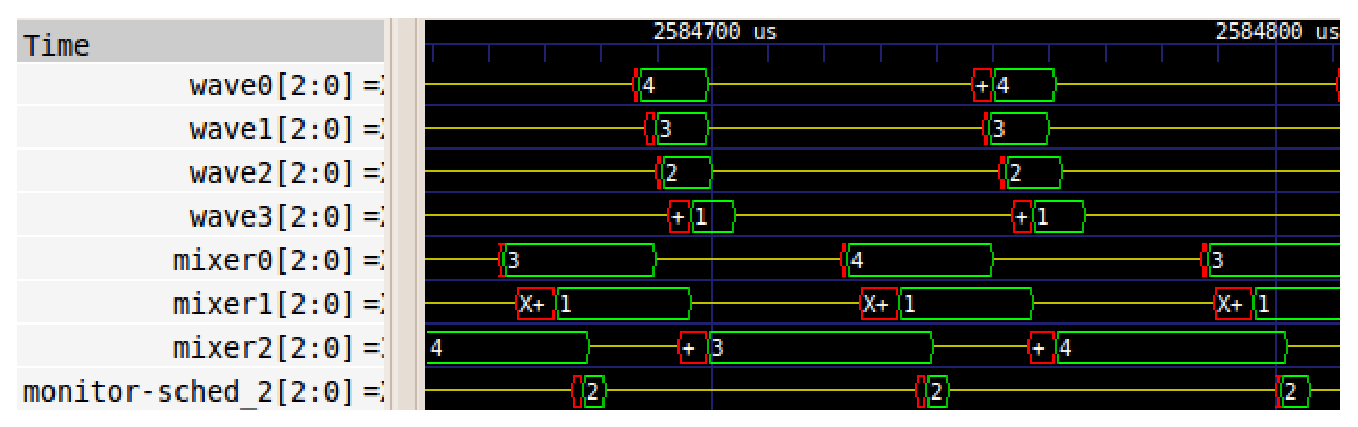
\includegraphics[width=\widefigure]{images/4KB_Xeon.eps}
\caption{\figurecaption{trace Xeon}}
\label{fig:trace_xeon}
\end{figure}

\begin{figure}[htbp]
\centering
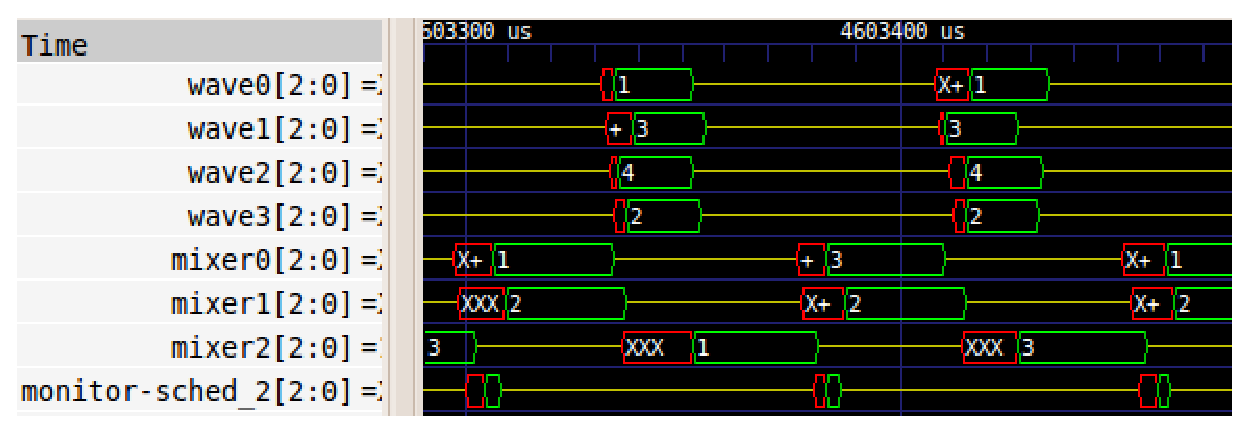
\includegraphics[width=\widefigure]{images/4KB_i7.eps}
\caption{\figurecaption{trace i7}}
\label{fig:trace_i7}
\end{figure}

\begin{figure}[htbp]
\centering
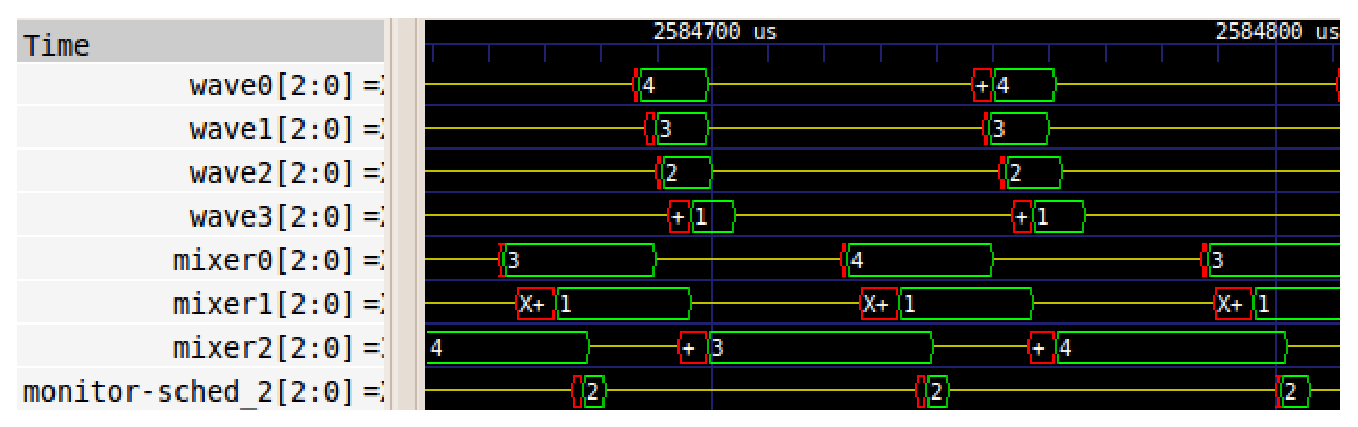
\includegraphics[width=\widefigure]{images/4KB_Xeon.eps}
\caption{\figurecaption{trace AMD}}
\label{fig:trace_xeon}
\end{figure}

\newpage

The following graphics visualize the average execution times of each task on different architecures using a buffer of 4KB 8KB 16KB 32KB 64KB

TODO graphic

The first difference that becomes immediately evident, is how the different architecture of i7 and Xeon influence performance of the application.
With 4KB, times on i7 increases by $~ 2x$ for waves, mixer0 and mixer1 have the about the same time of both architectures and mixer2 decreases its time by 
$~ 1.3x$. With others dimensions, times on i7 are worse than times on Xeon.

TODO AMD?

Another interesting difference is how change the time employed by mixers, on different architecture. On i7 execution time of mixer2 increase by $~ 5\%$ 
of the time of other mixers. On Xeon execution time of mixer2 increase more than $15\%$ of the time of other mixers.

On Intel Xeon, all task are not well parallelized because of overhead due to scheduling latency. The scheduling latency is the time interval that starts when
a task is enqeued on a runqueue and finish when it is executed \cite{lcs}. In \textit{trace} scheduling latency is time interval red-ink. To get a sense 
of how impact of scheduling latency change according to architecture see graphic in fig. TODO grafico sched lat

TODO grafico

TODO in didascalia This graphic was obtained measuring the average of scheduling latency and rapporting to average of exec time

There are many factors that influence scheduling latency. 


In the first place, inter-chip communication are different, Intel i7 use the new Quick-path 
Interconnect that is a point-to-point processor interconnect developed by Intel to compete with HyperTransport. This first implementation of this bus
achieve 25.6 GB/s, which provides exactly double the theoretical bandwidth of Intel's 1600 MHz FSB, that is the best performance obtainable with FSB.
From datasheet, Intel Xeon E5440 use a FSB at 1333 MHz. Cache architectures are different, Intel i7 uses three cache level and the LLC is shared among all 
processors, while Intel Xeon use two separated cache blocks and each block is shared among only two cpus, therefore communication bewtween cores that belong 
to different dies is very expensive. From these graphics is clear that on Intel Xeon a buffer of 4KB is not enough in order to neglect scheduling latency 
overhead.

\newpage

\begin{figure}[htbp]
\centering
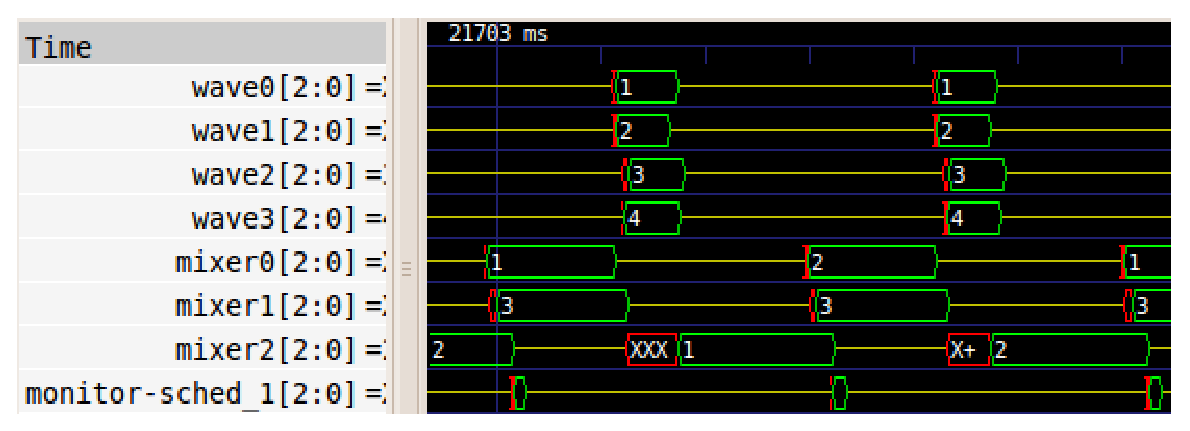
\includegraphics[width=\widefigure]{images/32KB_Xeon.eps}
\caption{\figurecaption{trace Xeon}}
\label{fig:trace_xeon}
\end{figure}

\begin{figure}[htbp]
\centering
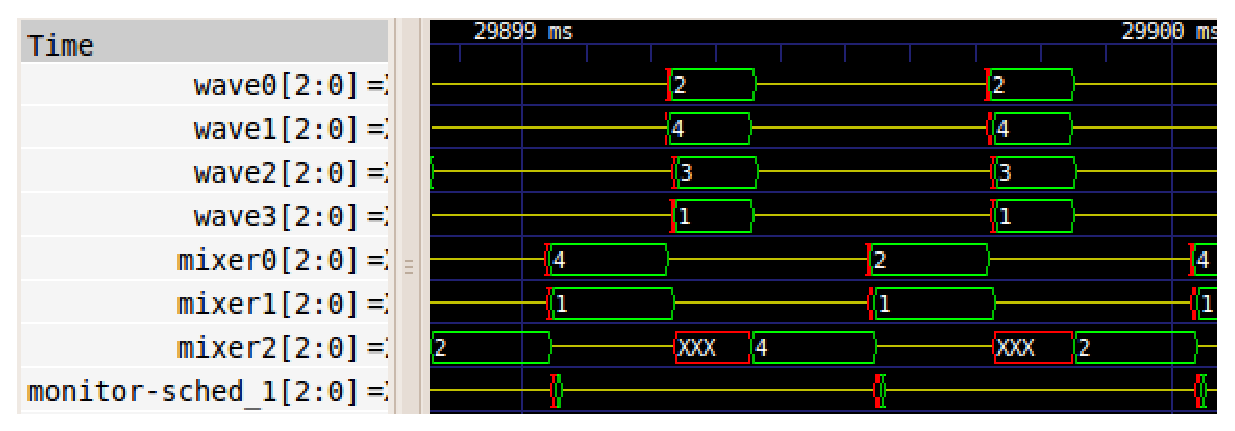
\includegraphics[width=\widefigure]{images/32KB_i7.eps}
\caption{\figurecaption{trace i7}}
\label{fig:trace_i7}
\end{figure}

\begin{figure}[htbp]
\centering
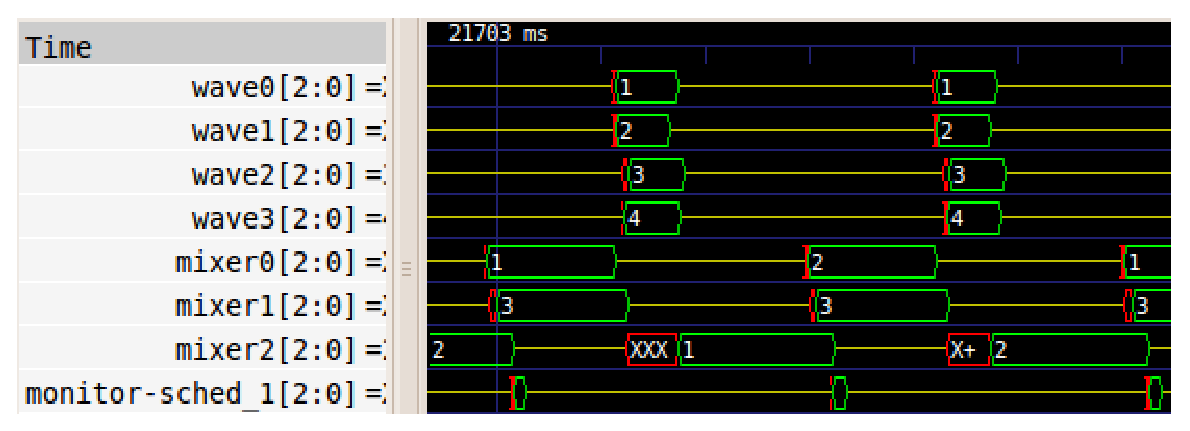
\includegraphics[width=\widefigure]{images/32KB_Xeon.eps}
\caption{\figurecaption{trace AMD}}
\label{fig:trace_xeon}
\end{figure}

\begin{figure}[htbp]
\centering
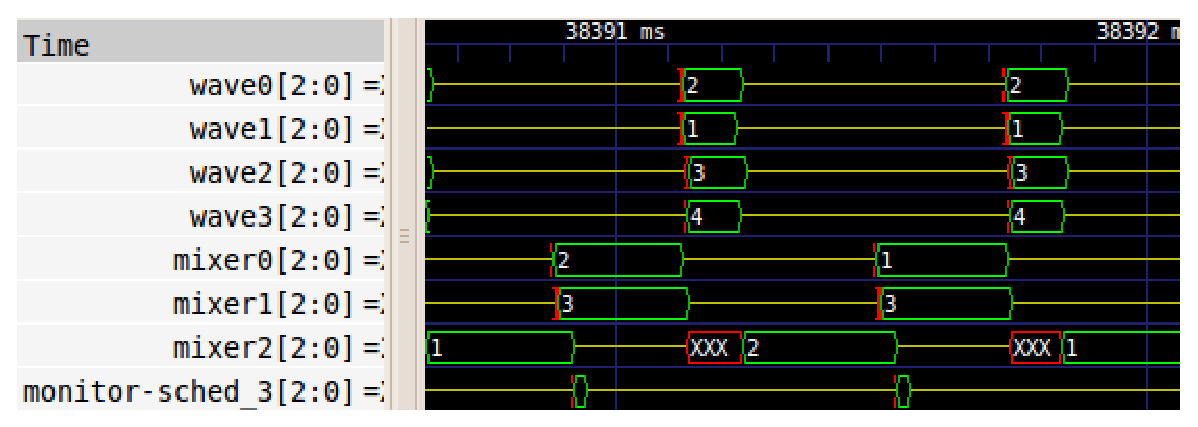
\includegraphics[width=\widefigure]{images/64KB_Xeon.eps}
\caption{\figurecaption{trace Xeon}}
\label{fig:trace_xeon}
\end{figure}

\begin{figure}[htbp]
\centering
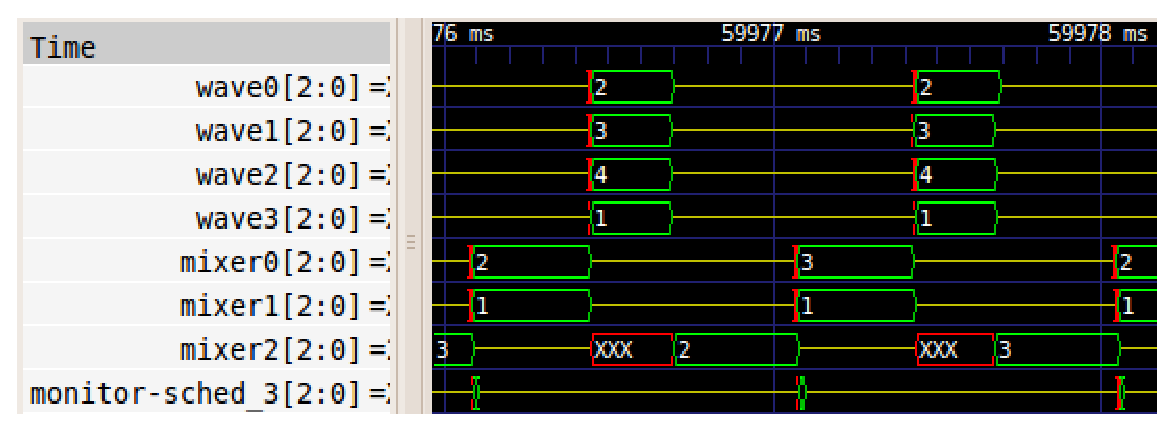
\includegraphics[width=\widefigure]{images/64KB_i7.eps}
\caption{\figurecaption{trace i7}}
\label{fig:trace_i7}
\end{figure}

\begin{figure}[htbp]
\centering
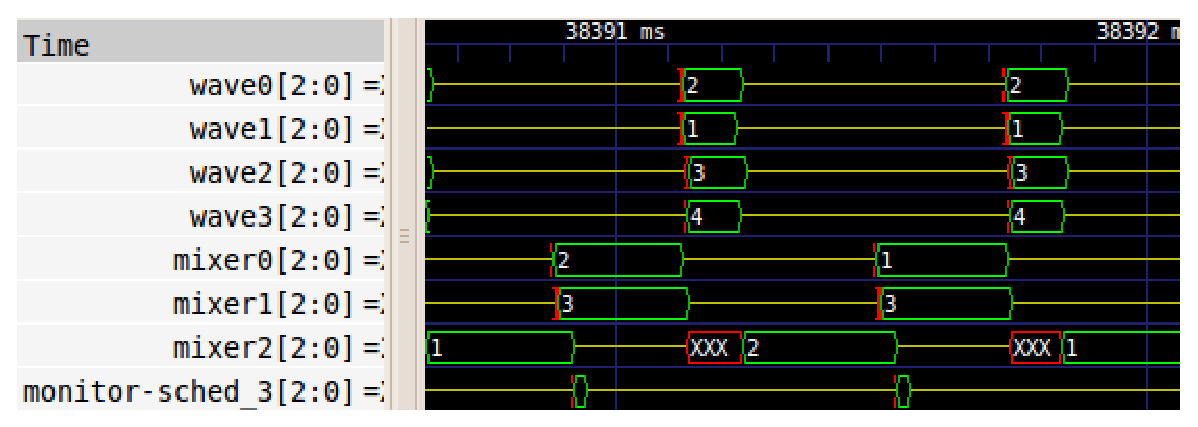
\includegraphics[width=\widefigure]{images/64KB_Xeon.eps}
\caption{\figurecaption{trace AMD}}
\label{fig:trace_xeon}
\end{figure}

\newpage

TODO dire che a queste dimensioni l\'overhead della sched latency viene meno, da verificare per\'o

%TODO il paragone dei tempi lo metterei alla fine del buffer size giustificandolo con la differenza di frequenze se c\'\'e davvero
TODO ricontrolla la storia dei tempi maggiori 


%-----------------------------------------------------------------------------
\subsection{Migration issues}

Unfortunately, current version of task-affinity is not very effective in term of reduction of task migrations. As already described in \cite{lcs}, during 
the benchmark's execution, the migration pattern showed in fig. TODO is verified

TODO trace con mig pattern

This problem is not related to the architecture used, it is an issue related to the logic of task-affinity. Consider the timestamp marked with orange line.
Mixer0 has to choice cpus that have executed Wave0 or Wave1 therefore it has to choice cpu1 or cpu2, Mixer1 has to choice cpu3 or cpu4, Mixer2 is in 
execution on cpu2. At marked timestamp, Mixer0 can't be executed on cpu2, that is on the last cpu that have executed it, because Mixer2 is still in 
execution on it, therefore mixer1 has to migrate. In general, any cpu Mixer0 or Mixer1 may choose, one of them will have to migrate, because they are 
waken up before that Mixer2 is finished and Mixer2 will always choose a cpu that have last executed mixer0 or Mixer1. 

Tasks's migration can degrade performance because a migrated task could warm up a new cache and it could create new cache interference in a new location 
already occupied by other tasks. 

In order to measure how much this migration pattern increase miss rate of the application, this experiment is performed:
Two run of benchmark are performed, in the first run all tasks are pinned on a specific cpu and they can't mirgate, the assignment is: 

\begin{itemize}
\item \textit{Wave0 -> cpu0}
\item \textit{Wave1 -> cpu1}
\item \textit{Wave2 -> cpu2}
\item \textit{Wave3 -> cpu3}
\item \textit{Mixer0 -> cpu0}
\item \textit{Mixer1 -> cpu2}
\item \textit{Mixer2 -> cpu2}
\end{itemize}

In the second run only waves are pinned on cpus 0 1 2 3. 

With this experiment it is possible to observe  TODO sperare che funzioni

TODO vale la pena farlo su tutti e tre?

TODO sta frase non so se buttarla, In our case warm up of cache shouldn't occurs because a mixer migrates always among the same cpus.

%-----------------------------------------------------------------------------
\subsection{Cache misses}

TODO menata dello Xeon ma solo per la L2 dicendo che per i banchdi divisi ci sar\'a sempre un miss da parte dei mixer ecc..

TODO dire come a 32KB la cache non conti niente


TODO dire che si deve migliorare la varianza
TODO capire chi migliora la varianza cache miss overhead migration (experiment cpuaffinity e task-affinity normale)
TODO profiler push e pull, dire che anche loro hanno importanza
TODO queste cose vanno qui perch\'e 


TODO i cache miss e le varianze

%-----------------------------------------------------------------------------
\subsection{profile push pull}

TODO dire che anche queste funzioni rompono il cazzo e incidono sulla varianza dell\'applicazione

Functions used to perform task migration influence the predictability of the application, especially when buffer dimension is greater or euqual to 32KB, 
because in that case, there isn't any improvement for cache misses and the variance of the execution time of these functions influence the predictability
of the application. 



TODO test per tutti e per le diverse dimensioni





%%%%%%%%%%%%%%%%%%%%%%%%%%%%%%%%%%%%%%%%%%%%%%%%%%%%%%%%%%%%%%%%%%%%%%%%%%%%%
\section{Task-affinity improvements}

Before to explain how the patch works, it is necessary to remember the concept of task-affinity. We say that two tasks have a task-affinity relationship if 
they share data and their execution depends upon reading or writing these data \cite{lcs}. In a producer-consumer application, the producer 
is the one that writes to the shared buffer, while the consumer is the one that reads it. The consumer depends on data generated by producer since it needs 
them in order to be able to run, therefore we say that the consumer has a task-affinity relationship toward the producer.

TODO img lcs

Each task is provided with a linked list called \textit{taskaffinity\_list} that contains all tasks to which it has task-affinity relationship, in briefly 
all its producers. To insert and delete a task in a \textit{taskaffinity list} two new system calls are provided:

\begin{description}

\item[sched\_add\_taskaffinity:]. This system call adds a dependency to the current task, i.e. the task that issued the call. It receives, as parameter, the 
pid of the task the current one will be dependent upon.

\item[sched\_del\_taskaffinity:]. When a task does not want anymore to use the task-affinity mechanism, it is possible to remove it through this call.
As in the case of inclusion of dependency, it suffices to pass as parameter the pid of the task one wants not to follow anymore.

\end{description}

Thanks to these system calls, the scheduler "knows" which tasks have task-affinity and, in this way, it can schedule consumers after producers in order to 
enforce reuse of cache memory.

The task-affinity logic influences wake up and migration of a task. As we have previously seen, in \textit{try\_to\_wake\_up} the choice of cpu where to 
put the to be waken task is made by \texttt{select\_task\_rq\_rt} TODO ref snip. This function is modified in this way: given the input task $p$, the 
function doesn't call \texttt{find\_lowest\_rq} but it loops for all element present in the $p$'s \textit{taskaffinity list} and build a mask, called 
\textit{affinity\_mask}, with cpus that have executed a task present in $p$'s \textit{taskaffinity list}. Finished the loop, the function returns the cpu 
with the runqueue that have the lowest number of Real-Time tasks. Only if the mask is empty, the function calls \texttt{find\_lowest\_rq} to choose a cpu
in the standard way. 

In the current version of task-affinity, a task that "respect" task-affinity, that is a task that was enqueued according to its task-affinity 
relationships, isn't able to migrate. In plain words, \texttt{push\_rt\_task} and \texttt{pull\_rt\_task} can't move tasks that "respect" task-affinity.

The aim of this policy is clear: when a task wakes up, the policy tries to select the best cpu for that task and, if it finds it, it blocks the task on the 
best runqueue until the task's execution. For this reason the key point of task-affinity logic is the \texttt{select\_task\_rq\_rt}. In the optimal case, 
producers and consumers will be executed subsequenlty always on the same cpu.

Nevertheless, in practice, the choosen cpu for $p$ is next to never the optimal cpu. The reason is very simple. The choice of the best 
cpu, and the enqueuing of task are performed in different moments. When \texttt{select\_task\_rq\_rt} is called, it doesn't held any lock. During the loop, 
the function has to read what is the content of different runqueues present in the system, these reads are not synchronized. When cpu is selected, 
\texttt{select\_task\_rq\_rt} returns, \texttt{try\_to\_wake\_up} \textbf{takes a lock} on choosen runqueue, in order to call \texttt{activate\_task} 
to perform the enqueuing of task. From when \texttt{select\_task\_rq\_rt} selects cpu to when lock is taken, a task with equal or higher priority than 
$p$'s priority can be inserted in the selected runqueue, in this way, the next task that will be executed won't be $p$. In figure TODO ref is represented 
this situation.

TODO img finestra temporale

The current version of task-affinity ensures a weak concept of temporal locality because it doesn't ensure, when it is possible, that the next task executed
after a producer is a consumer. Another problem of the current version of task-affinity is the migration policy. It is not quite flexible. Pull and push 
functions mantain the system balanced, and guarantee that every cpu executes always the higher priority Real-time task present in its runqueue.
Therefore, the deny to pull and push can improve predictability of the application and can degrade singnificantly the throughput of the application.
Predictability is an important aspect for Real-time systems, but if we have a very bad throughput we don't exploit the potentiality of multicore platforms.

The aim of the patch developed it to improve the concept of temporal locality and to improve the migration policy in order to use also the functions 
involved in the migration mechanism to exploit the concept of task-affinity. Furthermore, the patch make task-affinity more robust synchronizing access at 
data structures used.

%%%%%%%%%%%%%%%%%%%%%%%%%%%%%%%%%%%%%%%%%%%%%%%%%%%%%%%%%%%%%%%%%%%%%%%%%%%%%
\section{Patch structure}

TODO

%-----------------------------------------------------------------------------
\subsection{Temporal locality}

TODO Patch is optimized in wake migrattion.. say something

TODO temporal locality non come subsection ma come titolo in grassetto

TODO Temporal locality

To ensure that a consumer will be the next executed task after a producer, it is necessary to change what \texttt{select\_task\_rq\_rt} "see". As I 
previously said, during its loop, \texttt{select\_task\_rq\_rt} check for cpu that \textbf{have executed} a task in $p$'s \textit{taskaffinity list}. 
It means that, in that moment, those cpus could be executing a task that it is not a producer and then, L1 cache could be already dirty. For this reason, 
at each runqueue was added a field named \texttt{last\_tsk} that contains the last task executed in a runqueue. This field is updated at each context switch 
if the next task to be executed is different from idle. In this way, if current task on runqueue is not idle, this field represents, the task in execution. 

TODO figura last tsk

With this additional field, \texttt{select\_task\_rq\_rt} "knows" which is the task currently executed on each runqueue. In this way, cpus that during 
\texttt{select\_task\_rq\_rt} are executing a task that is not in $p$'s \textit{taskaffinity list} are not inserted in \texttt{affinity\_mask}.

This change is not enough. Consider this situation: two different cpus that we call CPU\_A and CPU\_B are executing two different istances of 
\texttt{try\_to\_wake\_up}. Respectively, they are called for task $p$ and task $q$: the former has task-affinity relationship, the latter is a generic 
Real-time task, both tasks have the same priority. Suppose that the current task on CPU\_A is a task in $p$'s \textit{taskaffinity list} and then 
\texttt{select\_task\_rq\_rt} choose CPU\_A for $p$. Suppose that \texttt{try\_to\_wake\_up} that wakes up $q$ chooses CPU\_A and enqueue task $q$ on 
runqueue of CPU\_A. Task $p$ is not still enqueued, therefore when it will be enqueued, it will be preceeded by $q$ and then the next task that will
be executed on CPU\_A is $q$.

TODO figura enqueue in testa

To resolve this problem, I have modified enqueuing of task in this manner: a task that "respects" task-affinity is enqueued on the top of a runqueue and not 
on tail. 

In this way, if two Real-time tasks are on the same runqueue and have the same priority, but one of them "respects" task-affinity, the next task that 
will be executed is the task that "respects" task-affinity. 

Until now we have modified the logic present in \texttt{try\_to\_wake\_up}. A carefully reader, will have noted that with this strategy a task with 
task-affinity can move up a task without task-affinity only if the latter is enqeued \textit{before} the former.

To resolve this problem, migration mechanism is used. When the \texttt{try\_to\_wake\_up} has enqueued task $p$, it calls \texttt{task\_woken} in order to
checks if $p$ can be executed on the selected runqueue or not. If on runqueue there is a task with priority equal or higher than the $p$'s priority and 
this task precede $p$, \texttt{push\_rt\_task} is called and $p$ can be pushed on another cpu. To select the cpu where to push $p$, the same mechanism used 
in \texttt{select\_task\_rq\_rt} is adopted. Therefore, $p$ will be pushed where it is in execution a task in $p$'s \textit{taskaffinity list}, if it is 
impossible standard push criteria are adopted and $p$ will be pushed on a cpu that executing a task with lower priority than $p$. Since now also 
\texttt{push\_rt\_task} is involved in task-affinity logic, and it use the same mechanism used in \texttt{select\_task\_rq\_rt},  the mechanism used to 
select taskaff TODO mettere il nome della funzione usata nella patch della find\_lowest. Obviously, in order to push a task that "respect" task-affinity, 
it is necessary insert it in a \textit{pushable list}. 


TODO alla fine faccio un riassunto magari lo metto in tabella

In the table TODO ref are reassumed change apported to current version of task-affinity, in order to improve temporal locality.

%-----------------------------------------------------------------------------
\subsection{Synchronization}


In the current version of task-affinity, accesses to data structures used to manage task-affinity are made by user or by kernel. The resource that must be
synchronized is \texttt{taskaffinity\_list} TODO del followme non sono sicuro

\begin{description}

\item[Access from user space:] User can access to task-affinity data structures using syscalls \texttt{sched\_add\_taskaffinity}, and 
\texttt{sched\_del\_taskaffinity}. These functions access to pid of the task received in input in synchronized way, because they using the read-write lock
tasklist\_lock that protects the kernel internal task list. For this reason, at every moment, only one instance of these syscalls can modify task-affinity 
data structure of a task.

TODO sezione di codice

\item[Access from kernel space:] Here the situation is more complex. There are two functions that can access to task-affinity data structures, they are:
\texttt{task\_affinity\_notify\_exit} and \texttt{select\_task\_rq\_rt}. The former function frees task-affinity data structures and it is called when a 
task is exiting. During this phase, all resources used by a task, pid included, are deallocated therefore, when \texttt{task\_affinity\_notify\_exit} is 
called, \textit{tasklist\_lock} is acquired. This is not enough because in that moment \texttt{select\_task\_rq\_rt} can access to task-affinity data 
structure of the exiting task, for this reason another layer of synchronization is needed. To resolve this problem, each task has its own read-write lock 
named \textit{taskaff\_lock} to protect its task-affinity data structures. 

\end{description}

TODO immagine accesso alle strutture dati

In figure are represented the two step of sycnhronization. In step (a) syscalls try to acquire \textit{tasklist\_lock} in order to avoid to access to a 
\textit{taskaffinity list} of an exiting task. In step (b) all functions that want to access to task-affinity data structure of a certain task, must 
acquire the \textit{taskaff\_lock} that protect those structures. A read-write lock was choosen because reads on task-affinity data structures are 
most frequently than writes. Reads are performed by \texttt{select\_task\_rq\_rt} while writes are executed only by the syscalls and 
\texttt{task\_affinity\_notify\_exit}.


TODO  alla fine della sezione metto il commento della legge di amdhal che ha fatto lcs per dire quello che lui ipotizza lo scheduler che ha fatto
io invece dico che voglio anticipare quindi lo speed up \'e differente ecc.
